\documentclass{article}
\usepackage[a4paper, tmargin=1in, bmargin=1in]{geometry}
\usepackage[utf8]{inputenc}
\usepackage{graphicx}
\usepackage[justification=centering]{caption}

% \usepackage{parskip}
\usepackage{amsmath}
\usepackage{siunitx}
\sisetup{round-mode=places, round-precision=4}
\usepackage{ bbold }

\usepackage{pdflscape}
\usepackage{listings}
\usepackage{hyperref}
\usepackage{caption}
\usepackage{subcaption}
\usepackage{float}

\title{EE 771 : Recent Topics in Analytical Signal Processing Assignment 1}
\author{Arka Sadhu - 140070011}
\date{\today}

\begin{document}
\maketitle

\section*{Q1}
\subsection*{1a}
% \newcolumntype{X}{D{.}{.}{1,3}}
Eigen Vectors ordered by Eigen Values \\
$
\begin{bmatrix}
  0.378 & 0.449 & 0.000 & 0.000 & -0.280 & 0.752 & -0.111 \\
  0.378 & 0.637 & 0.000 & 0.000 & 0.569 & -0.355 & 0.027 \\
  0.378 & 0.128 & 0.000 & 0.000 & -0.711 & -0.484 & 0.316 \\
  0.378 & -0.231 & 0.000 & 0.000 & -0.083 & -0.211 & -0.868 \\
  0.378 & -0.328 & 0.365 & 0.816 & 0.168 & 0.099 & 0.212 \\
  0.378 & -0.328 & -0.815 & -0.408 & 0.168 & 0.099 & 0.212 \\
  0.378 & -0.328 & 0.450 & -0.408 & 0.168 & 0.099 & 0.212
\end{bmatrix}
$
\subsection*{1b}
Coordinates of f in the above basis \\
$
\begin{bmatrix}
  4.536 & 2.240 & 1.180 & 1.633 & 1.242 & 2.653 & 1.506 \\
\end{bmatrix}
$
\subsection*{1c}

\begin{figure}[H]
  \centering
  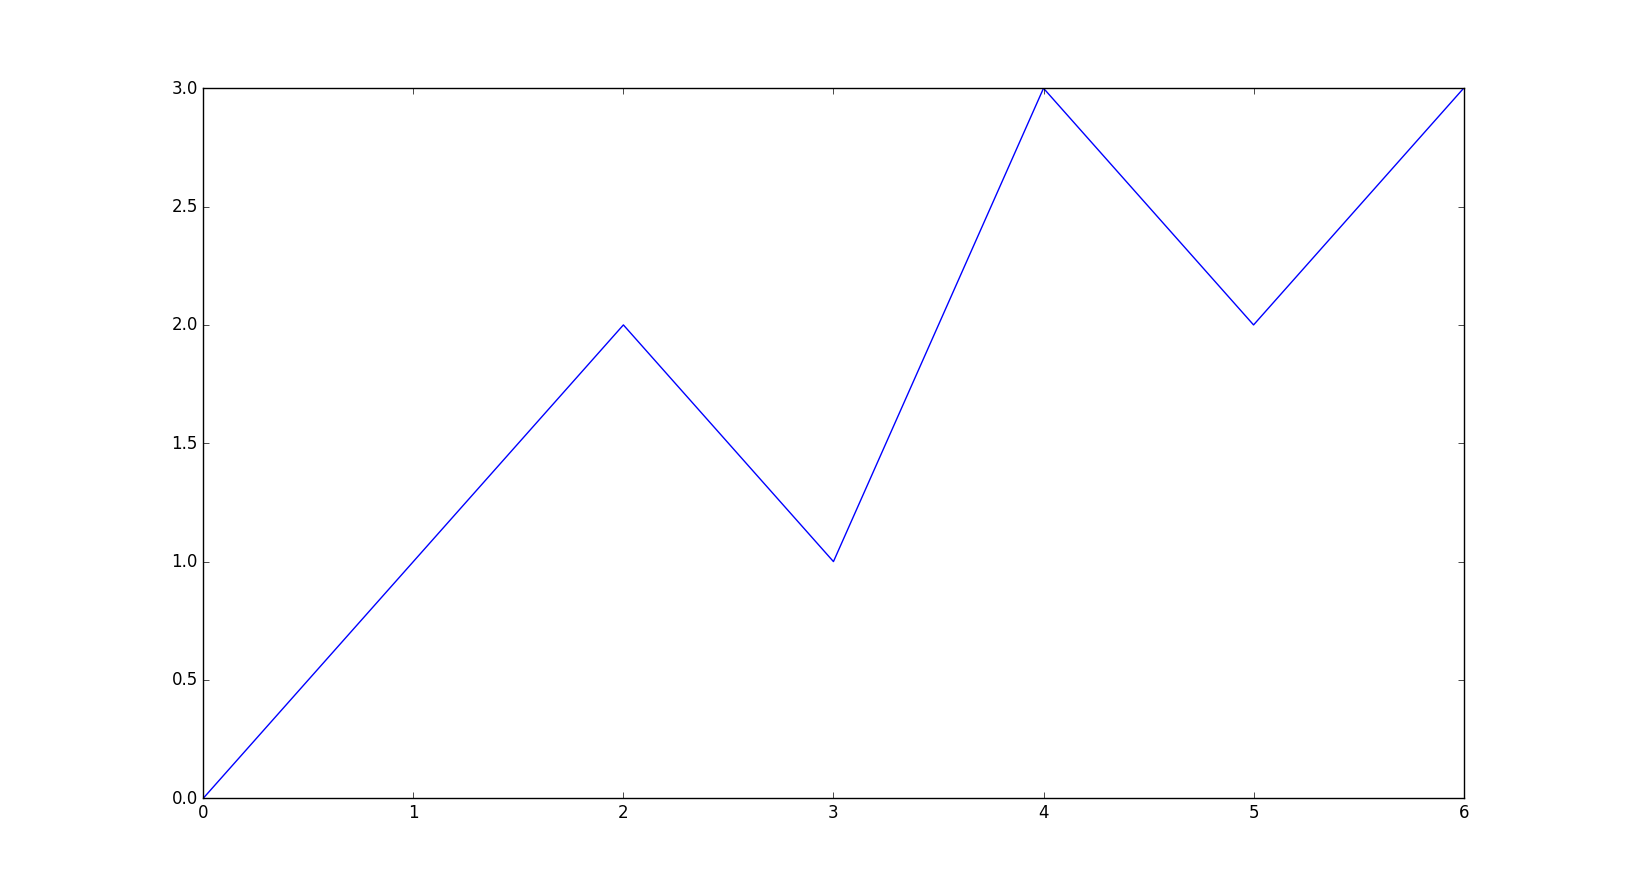
\includegraphics[scale=0.25]{images/q1c_zero_cross}
  \caption{Number of Zero Crossing in the Eigen Vectors}
  \label{fig:q1c}
\end{figure}

In vector form for easier representation the number of zero crossing are: \\
$\begin{bmatrix}
  0. & 1. & 2. & 1. & 3. & 2. & 3.
\end{bmatrix}
$

\subsection*{1d}
Original Graph Signal f in vector form :\\
$ f =\begin{bmatrix}
  3. & 1. & 2. & 2. & 2. & 1. & 1.
\end{bmatrix}$
Low Pass Graph Signal f after retaining only the four eigen vectors corresponding to the smallest four eigen values.\\
$f_L =
\begin{bmatrix}
    1.924 & 2.012 & 1.774 & 1.606 & 2.361 & 0.930 & 1.392
\end{bmatrix}
$

We note that in the reconstructed signal which is basically the original signal passed through a low pass filter in the graph fourier domain has lesser variation than that in the original signal since we removed the components along high frequency eigen vectors.

\section*{Q2}
\begin{figure}[H]
  \centering
  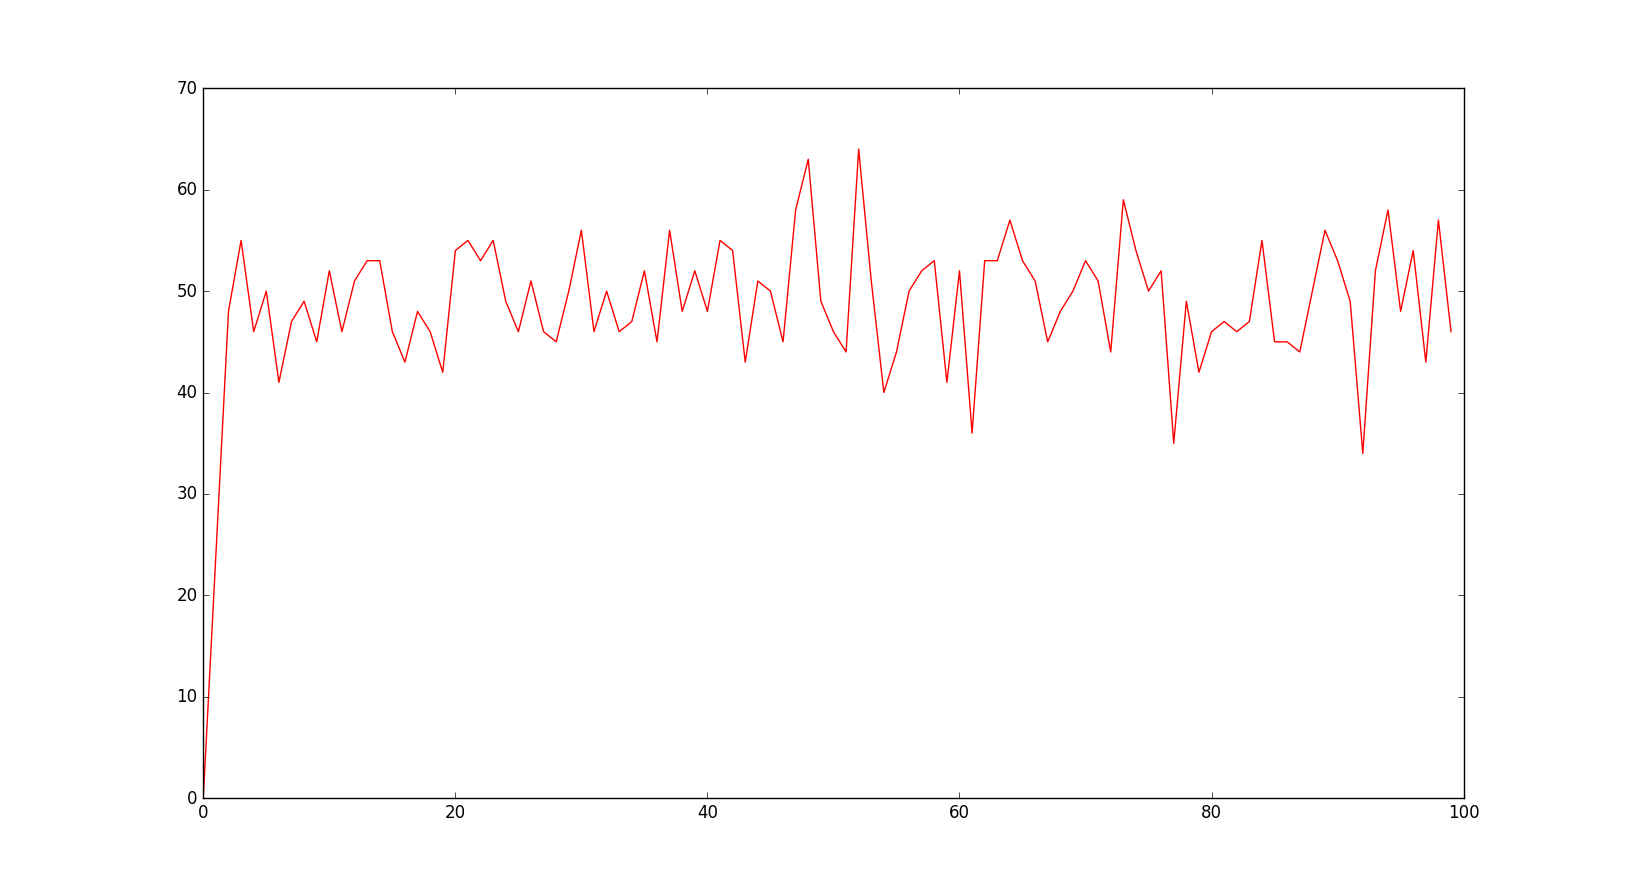
\includegraphics[scale=0.25]{images/q2_num_zero_cross}
  \caption{Zero Crossing for Eigen Vectors of Laplacian Matrix for ER graph. Here x-axis is the index of the eigenvector in increasing order or eigenvalue. y-axis is the number of zero crossing in the corresponding eigen vector}
  \label{fig:q2}
\end{figure}

Observation:
\begin{itemize}
\item First we note that  the number of zero crossing is 0 for the first eigenvector as contains the same value in all its indices and corresponds to the 0 eigen value.
\item Next we note that there is rapid increase in the number of zero crossing in the first few eigen vectors. This is consistent with the corresponding observation in usual digital signal processing that higher indices correspond to higher frequency.
\item We also note that the number of zero crossing fluctuates between consecutive eigen vectors but is consistently above a minimum threshold and below some maximum threshold. This seems to suggest some form of saturation of the highest frequency being achieved in some sense and doesn't have an analog in the usual DSP sense.
\end{itemize}

\section*{Q3}
\begin{figure}[H]
  \centering
  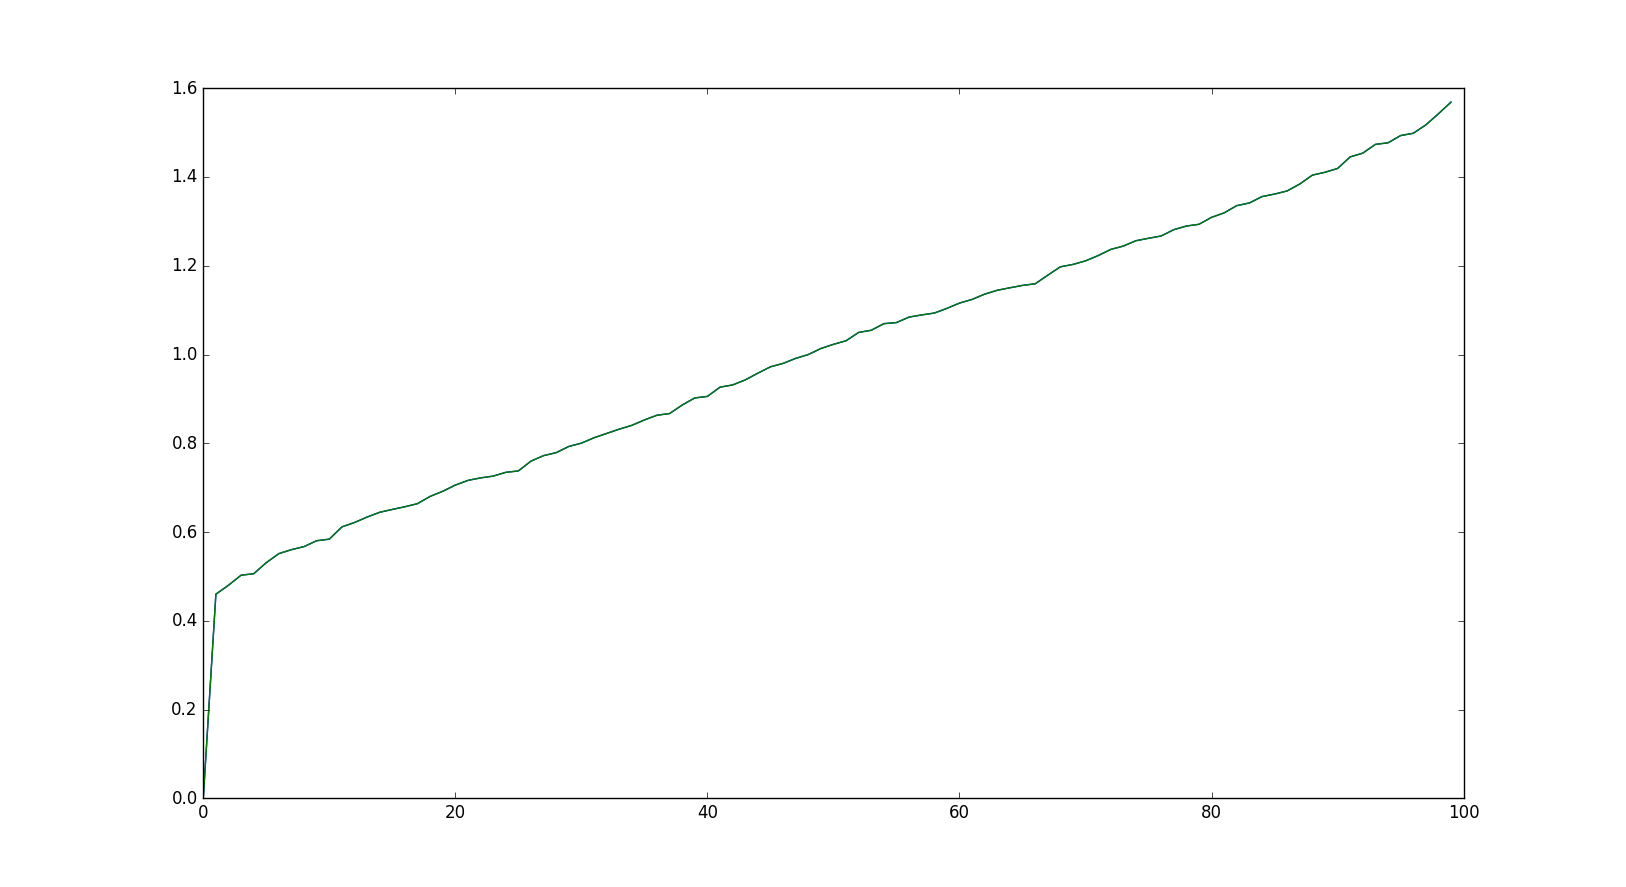
\includegraphics[scale=0.25]{images/q3_eig_vals}
  \caption{Plot of EigenValues sorted vs the index for the Normalized Laplacian}
  \label{fig:q3}
\end{figure}

Comments:
\begin{itemize}
\item It is noted that the eigenvalues of the normalized Laplacian are bounded in the range [0, 2].
\item It appears that the initial increase in eigen value is quite steep, and after some fixed index increases in a linear fashion with a constant slope.
\end{itemize}

\section*{Q4}
Image denoising. Parameters chosen for good denoising (different from those stated in the paper). $\theta = 1$ and $\kappa = 1.5$.

$\theta = 0.1$ is not chosen as it led to the weight matrix and corresponding laplacian to have extremely small values leading to eigenvalues with very small values. $\kappa = 1.5$ is chosen to accomodate weights even for diagonal connections as well.

\begin{figure}[H]
  \centering
  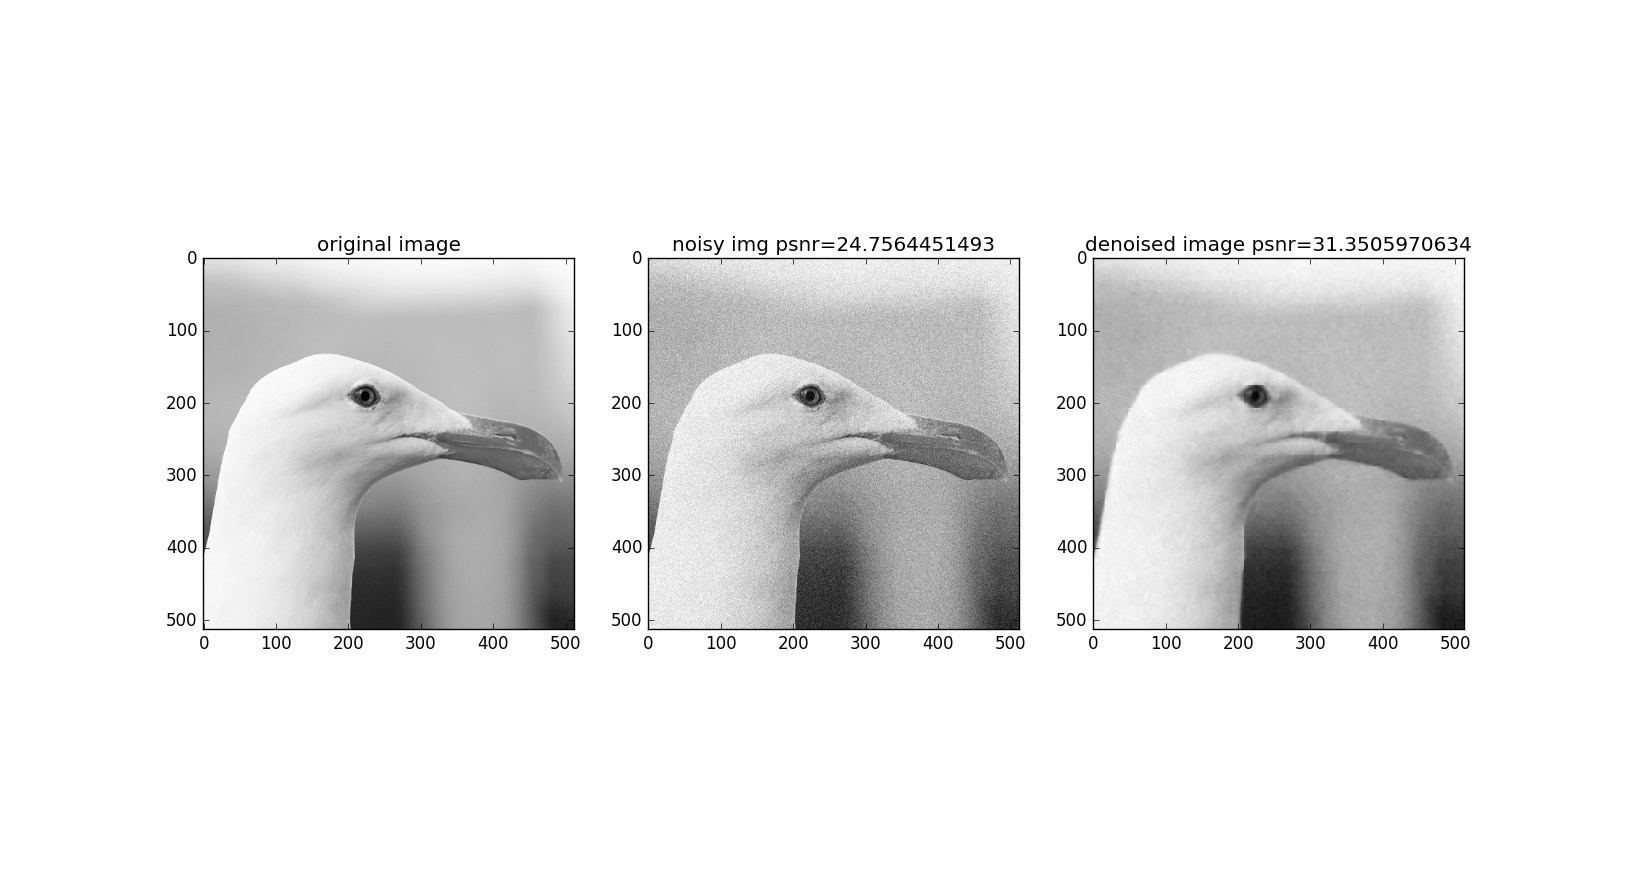
\includegraphics[scale=0.4]{images/q4_1_denoise}
  \caption{Image Denoising for SeaGull}
  \label{fig:q4_1}
\end{figure}

\begin{figure}[H]
  \centering
  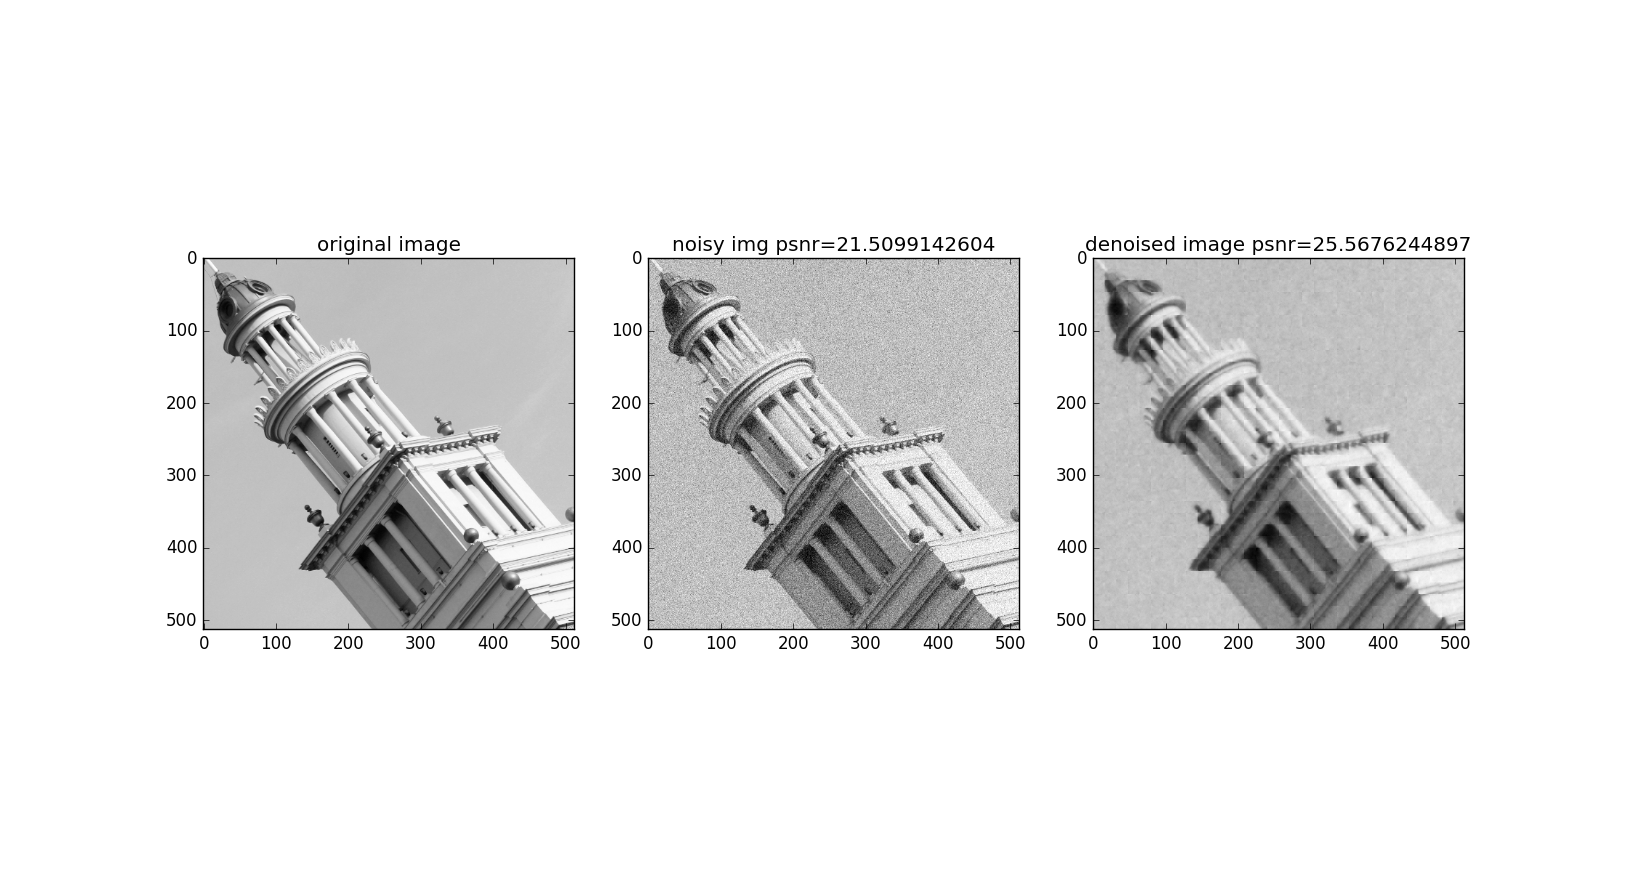
\includegraphics[scale=0.4]{images/q4_2_denoise}
  \caption{Image Denoising for sko}
  \label{fig:q4_2}
\end{figure}

We note that in both cases the psnr of the denoised image is considerably higher than that of the noisy image and therefore the low pass based on graph fourier transform indeed works as intended.

\section*{Q5}
$Eigen Vectors =  \\
\begin{bmatrix}
  0.408 & 0.210 & -0.577 & 0.577 & 0.218 & 0.408 \\
  0.408 & -0.571 & 0.289 & -0.289 & -0.572 & 0.408 \\
  0.408 & 0.361 & 0.289 & -0.289 & 0.354 & 0.408 \\
  0.408 & 0.571 & -0.289 & -0.289 & -0.572 & -0.408 \\
  0.408 & -0.361 & -0.289 & -0.289 & 0.354 & -0.408 \\
  0.408 & -0.210 & 0.577 & 0.577 & 0.218 & -0.408
\end{bmatrix}$

And the corresponding Eigen Values:
$Eigen Values = \\
\begin{bmatrix}
  0.0 & 0.5 & 0.5 & 1.5 & 1.5 & 2.0
\end{bmatrix}
$

Checking Symmetry Properties:
\begin{itemize}
\item We firstly note that normalized laplacian matrix has been used, therefore the eigenvalues lie in the range [0, 2].
\item Next we note that when $\lambda$ is an eigenvalue, $2-\lambda$ is also an eigen value. The pairs here are : $[(0, 2), (0.5, 1.5), (0.5, 1.5)]$. This is because of the graph is bipartite with the partitions H=[1,2,3] and L=[4,5,6]
\item We further note that the eigen vectors have the property that: if
  $u = \begin{bmatrix}
    u_H \\
    u_L \\
  \end{bmatrix}$
  is the eigenvector corresponding to the eigenvalue say $\lambda$ then the eigenvector
  $v =
  \begin{bmatrix}
    u_H \\
    -u_L\\
  \end{bmatrix}$
  corresonds to the eigenvalue $2-\lambda$.
\item For the eigen pair (0, 2) the eigenvectors are
  $u_0 =
  \begin{bmatrix}
      0.408 & 0.408 & 0.408 & 0.408 & 0.408 & 0.408
    \end{bmatrix}$
    and
    $u_5 =
    \begin{bmatrix}
        0.408 & 0.408 & 0.408 & -0.408 & -0.408 & -0.408
    \end{bmatrix}$

    Similarly for the pairs (0.5, 1.5) the eigen vectors are
    $u_1 =
    \begin{bmatrix}
      0.210 & -0.571 & 0.361 & 0.571 & -0.361 & -0.210
    \end{bmatrix}$
    and
    $u_4 =
    \begin{bmatrix}
      0.218 & -0.572 & 0.354 & -0.572 & 0.354 & 0.218
    \end{bmatrix}$

    And the remaining pair (0.5, 1.5) we have :
    $u_2 =
    \begin{bmatrix}
      -0.577 & 0.289 & 0.289 & -0.289 & -0.289 & 0.577
    \end{bmatrix}$
    and
    $u_3 =
    \begin{bmatrix}
        0.577 & -0.289 & -0.289 & -0.289 & -0.289 & 0.577
    \end{bmatrix}$

\item The downsampled versions of $f_L$ and $f_H$ are given by
 $$f_L = \frac{1}{2} (I + J_{\beta_L}) f$$
 $$f_H = \frac{1}{2}(I + J_{\beta_H}) f$$
Here $\beta_H$ is a vector indexed by the node number. $\beta_H[n] = \mathbb{1}_{n \in H} - \mathbb{1}_{n \in L}$. It is easy to note that $\beta_L = - \beta_H$. $J_{\beta_H}$ and $J_{\beta_L}$ are correspondingly diagonalization of the corresponding $\beta$.

\item In this case we find $f_L =
  \begin{bmatrix}
    0. & 0. & 0. & 1. & 2. & 3.
  \end{bmatrix}$
  and
  $f_H =
  \begin{bmatrix}
    1. & 2. & 3. & 0. & 0. & 0.
  \end{bmatrix}$


\end{itemize}
\end{document}
